\documentclass[t,usepdftitle=false]{beamer}

\usepackage[utf8]{inputenc}
\usetheme{Singapore}
\usepackage{xcolor}

% \setbeamercovered{transparent}
%\usecolortheme{crane}
\title[Méthode du simplexe]{Programmation Linéaire\\Méthode du simplexe}
\author[Fabian Bastin]{Fabian Bastin\\DIRO\\Université de Montréal}
\date{}

\usepackage{ulem}
\usepackage{tikz}
\newcommand*\circled[1]{\tikz[baseline=(char.base)]{
    \node[shape=circle,draw,inner sep=2pt] (char) {#1};}}

\def\ba{\boldsymbol{a}}
\def\bb{\boldsymbol{b}}
\def\bc{\boldsymbol{c}}
\def\be{\boldsymbol{e}}
\def\br{\boldsymbol{r}}
\def\bx{\boldsymbol{x}}
\def\by{\boldsymbol{y}}
\def\bz{\boldsymbol{z}}
\def\bA{\boldsymbol{A}}
\def\bB{\boldsymbol{B}}
\def\bD{\boldsymbol{D}}
\def\bzero{\boldsymbol{0}}

\def\cR{\boldsymbol{R}}
\def\RR{\mathbb{R}}

\setbeamertemplate{footline}[frame number]

\begin{document}
\frame{\titlepage}

% ------------------------------------------------------------------------------------------------------------------------------------------------------\begin{frame}
\begin{frame}
\frametitle{La méthode du simplexe}

Principe général: visiter de manière ``intelligente'' les points extrêmes de l'ensemble réalisable.

\mbox{}

``Intelligent'': chaque point extrême nouvellement visité devrait correspondre à une valeur plus petite de la fonction objectif.

\end{frame}
% ------------------------------------------------------------------------------------------------------------------------------------------------------\begin{frame}
\begin{frame}
\frametitle{Pivots: première interprétation}

Considérons l'ensemble d'équations
\begin{align*}
a_{11}x_1 + a_{12}x_2 + \ldots + a_{1n}x_n &= b_1 \\
a_{21}x_1 + a_{22}x_2 + \ldots + a_{2n}x_n &= b_2 \\
\qquad \vdots \\
a_{m1}x_1 + a_{m2}x_2 + \ldots + a_{mn}x_n &= b_m
\end{align*}
avec $m \leq n$.

\mbox{}

Sous forme matricielle, on peut écrire
\[
\bA \bx = \bb.
\]

\end{frame}

\begin{frame}
\frametitle{Pivots: première interprétation}

Dénotons par $\ba^i$ la $i^e$ ligne de $\bA$. Cela donne
\begin{align*}
\ba^1 \bx &= b_1 \\
\ba^2 \bx &= b_2 \\
\qquad \vdots \\
\ba^m \bx &= b_m
\end{align*}

\end{frame}

\begin{frame}
\frametitle{Pivots: première interprétation}

Si $m < n$ et que les équations sont linéairement indépendantes  (i.e. rang($A$) = $m$), il n'y a pas une solution unique mais une variété linéaire de solutions.

\mbox{}

Note: un ensemble $V$ dans $E^n$ est dit {\color{blue}variété linéaire} si pour tout $\bx_1$, $\bx_2$ appartenant à V, et pour tout réel $\alpha$, $\alpha \bx_1 + (1-\alpha)\bx_2$ appartient \`a V.

\mbox{}

En effet, si $\bx_1$ and $\bx_2$ sont des solutions satisfaisant
$$
\bA\bx_1 = \bb, \qquad \bA\bx_2 = \bb,
$$
alors pour tout $\alpha \in \RR$,
$$
\bA(\alpha \bx_1 + (1-\alpha) \bx_2) = \alpha \bA\bx_1 + (1-\alpha) \bA\bx_2 = \bb.
$$

\end{frame}

\begin{frame}
\frametitle{Pivots: première interprétation}

$m < n$, équations linéairement indépendantes.

\mbox{}

On peut ajouter $n-m$ équations de la forme
\[
\be^k x = 0,
\]
avec
\[
 \begin{matrix} \be^k = ( & 0 & \ldots & 0, \underbrace{1}_{k^e \mbox{ position}} & 0 & \dots & 0 & )^T \end{matrix}.
\]

\mbox{}

Ceci revient à fixer $x_k$ à 0, vu que
\[
\be^k x = 0 \Leftrightarrow x_k = 0.
\]
En procédant de la sorte, on obtient une solution de base au système linéaire.

\mbox{}

Différentes solutions de base seront obtenues en imposant différentes équations additionnelles de cette forme.

\end{frame}

\begin{frame}
\frametitle{Exemple}

On considère le problème
\begin{align*}
\min_x \ & 6x_1 + 3x_2 - x_3 + x_4 \\
\mbox{t.q. } & x_1 + x_2 = 4 \\
& x_2 - x_3 = 2; \\
& x_1, x_2, x_3, x_4 \in \RR^+.
\end{align*}

\mbox{}

\[
A = \begin{pmatrix}
1 & 1 & 0 & 0 \\
0 & 1 & -1 & 0 \\
\end{pmatrix}
\]
Dès lors,
\[
a_1 = \begin{pmatrix} 1 \\ 0 \end{pmatrix}
\quad
a_2 = \begin{pmatrix} 1 \\ 1 \end{pmatrix}
\quad
a_3 = \begin{pmatrix} 0 \\ -1 \end{pmatrix}
\quad
a_4 = \begin{pmatrix} 0 \\ 0 \end{pmatrix}
\]
Une base ne pourra faire intervenir que $a_1$, $a_2$ et $a_3$.

\end{frame}

\begin{frame}
\frametitle{Exemple}

Prenons $a_1$ et $a_3$ pour composer la base. On complète $A$ avec $e^2$ et $e^4$.
\[
\begin{pmatrix}
1 & 1 & 0 & 0 \\
0 & 1 & -1 & 0 \\
0 & 1 & 0 & 0 \\
0 & 0 & 0 & 1
\end{pmatrix}
\]
et on considère le système
\[
\begin{pmatrix}
1 & 1 & 0 & 0 \\
0 & 1 & -1 & 0 \\
0 & 1 & 0 & 0 \\
0 & 0 & 0 & 1
\end{pmatrix}
\begin{pmatrix}
x_1 \\ x_2 \\ x_3 \\ x_4
\end{pmatrix}
=
\begin{pmatrix}
4 \\ 2 \\ 0 \\ 0
\end{pmatrix}
\]
Mais la base n'est pas réalisable!

Le système a pour solution $(4, 0, -2, 0)$.
\end{frame}

\begin{frame}
\frametitle{Forme canonique}

\textbf{\textcolor{red}{Définitions}}
\begin{itemize}
\item
une variable est \textcolor{blue}{isolée} si son coefficient est égal à 1 dans une équation et zéro dans les $m-1$ autres équations
\item
un système est sous \textcolor{blue}{forme canonique} s'il contient (au moins) $m$ variables isolées.
\end{itemize}

Supposons s.p.d.g. que les $m$ premières variables sont isolées, donnant le système sous forme canonique
\[
\begin{matrix}
x_1 & & \ & & +\ y_{1,m+1}x_{m+1} +\ y_{1,m+2}x_{m+2} +\ \ldots +\ y_{1,n}x_{n} = y_{10} \\
& x_2 & & & +\ y_{2,m+1}x_{m+1} +\ y_{2,m+2}x_{m+2} +\ \ldots +\ y_{2,n}x_{n} = y_{20} \\
& & & & & \vdots \\
& & & x_m & +\ y_{m,m+1}x_{m+1} +\ y_{m,m+2}x_{m+2} +\ \ldots +\ y_{m,n}x_{n} = y_{m0}
\end{matrix}
\]
\end{frame}

\begin{frame}
\frametitle{Forme canonique}

Sous forme matricielle, nous pouvons réécrire le système comme
$$
\begin{pmatrix}
I &  D
\end{pmatrix}
\begin{pmatrix}
x_1 \\ \vdots \\ x_m \\ x_{m+1} \\ \vdots \\ x_n
\end{pmatrix} =
\begin{pmatrix}
y_{10} \\ \vdots \\ y_{m0}
\end{pmatrix}
$$
ou encore
$$
\begin{pmatrix}
x_1 \\ \vdots \\ x_m
\end{pmatrix}
+
D
\begin{pmatrix}
x_{m+1} \\ \vdots \\ x_n
\end{pmatrix} =
\begin{pmatrix}
y_{10} \\ \vdots \\ y_{m0}
\end{pmatrix}
$$
\end{frame}

\begin{frame}
\frametitle{Forme canonique -- solution de base}

Posons
$x_{m+1} = \ldots = x_n = 0$ et
$$
\begin{pmatrix}
x_1 \\ \vdots \\ x_m
\end{pmatrix}
=
\begin{pmatrix}
y_{10} \\ \vdots \\ y_{m0}
\end{pmatrix}
$$

Nous avons la solution de base
$$
\bx = (\by_0, 0),
$$
avec $\by_0 = (y_{10},y_{20},\ldots,y_{m0})$

\mbox{}

Mais ce n'est qu'une solution de base parmi d'autres!

\mbox{}

$x_1$, $x_2$, \ldots, $x_m$: variables de base\\
$x_{m+1}$, $x_{m+2}$, \ldots, $x_n$: variables hors base

\end{frame}

%\begin{frame}
%\frametitle{Pivots: forme canonique}

%Si les équations sont linéairement dépendantes, on peut remplacer une équation par un multiple non-nul d'elle-même plus une combinaison linéaire des autres lignes du systèmes.

%\mbox{}

%{\color{blue}But}: réduire le système à la forme canonique.

%\mbox{}

%{\color{blue}Note}: on suppose ici que les variables de base sont les $m$ premières variables pour la simplicité de l'exposition, mais en pratique, cela peut être n'importe quel ensemble de $m$ variables.

%\end{frame}

\begin{frame}
\frametitle{Pivots: solution de base}

{\color{blue}But}: réduire le système à la forme canonique.

\mbox{}

Représentation du système comme un \textit{tableau} de coefficients:
\[
\begin{matrix}
1 & 0 & \cdots & 0 & y_{1,m+1} & y_{1,m+2} & \cdots & y_{1n} & y_{10} \\
0 & 1 & \cdots & 0 & y_{2,m+1} & y_{2,m+2} & \cdots & y_{2n} & y_{20} \\
0 & 0 & \cdots & 0 & y_{3,m+1} & y_{3,m+2} & \cdots & y_{3n} & y_{30} \\
\vdots & \vdots & \ddots & \vdots & \vdots & \vdots & \ddots & \vdots & \vdots \\
0 & 0 & \cdots & 1 & y_{m,m+1} & y_{m,m+2} & \cdots & y_{mn} & y_{m0}
\end{matrix}
\]

\mbox{}

Principe du pivot: \textcolor{red}{échanger une variable hors base avec une variable de base}.

\mbox{}

Supposons que nous voulons remplacer la variable de base $x_p$, $1 \leq p \leq m$, par la variable hors base $x_q$, $m < q$.

\mbox

Ceci est possible si et seulement si $y_{pq} \ne 0$, appelé {\sl élément pivot}.

\end{frame}

\begin{frame}
\frametitle{Pivot}

Divisons par $y_{pq}$ la $p^e$ équation:
%\[
%0 \ \cdots \ 0 \ \frac{1}{y_{pq}} \ 0 \ \cdots \ 0 \ \frac{y_{p,m+1}}{y_{pq}} \ \frac{y_{p,m+1}}{y_{pq}} \ \frac{y_{p,m+2}}{y_{pq}} \  \cdots \ \frac{y_{pq}}{y_{pq}} \ \ldots \ \frac{y_{pn}}{y_{pq}} \  \frac{y_{p0}}{y_{pq}}
%\]
\setcounter{MaxMatrixCols}{20}
$$
\begin{matrix}
0 & \cdots & 0 & \frac{1}{y_{pq}} & 0 & \cdots & 0 & \frac{y_{p,m+1}}{y_{pq}} & \frac{y_{p,m+1}}{y_{pq}} & %\frac{y_{p,m+2}}{y_{pq}} &
\cdots & \frac{y_{pq}}{y_{pq}} & \ldots & \frac{y_{pn}}{y_{pq}} & \frac{y_{p0}}{y_{pq}}
\end{matrix}
$$
Le coefficient de $x_q$ vient de passer à 1 dans cette équation.

\mbox{}

En d'autres termes, la $p^e$ ligne devient
$$
 y'_{pj} = \frac{y_{pj}}{y_{pq}}.
$$

\mbox{}

Il reste à supprimer cette variable des autres équations, en mettant à 0 le coefficient de $x_q$ dans les autres lignes du système.

\end{frame}

\begin{frame}
\frametitle{Pivot}

\begin{itemize}
\item
Pour mettre à 0 les coefficients dans les autres lignes, on va enlever le multiple adéquat de la $p^e$ ligne.
\item
Ainsi, pour $i \ne p$, on prend
$$
y'_{ij} = y_{ij} - \frac{y_{pj}}{y_{pq}} y_{iq}.
$$
\item
En particulier, nous avons alors $y'_{iq} = 0$ pour $i \ne p$.
\end{itemize}

\end{frame}

\begin{frame}
\frametitle{Exemple}

On considère le système sous forme canonique
\begin{eqnarray*}
x_1 & & \quad + x_4 +  x_5 - x_6 = 5 \\
& x_2 & \quad + 2x_4 -3x_5 + x_6 = 3 \\
& & x_3 -x_4 +2x_5 - x_6 = -1
\end{eqnarray*}

Sous forme de tableau, nous avons
\[
\begin{matrix}
x_1 & x_2 & x_3 & x_4 & x_5 & x_6 & \\
1 & 0 & 0 & \circled{1} & 1 & -1 & 5 \\
0 & 1 & 0 & 2 & -3 & 1 & 3 \\
0 & 0 & 1 & -1 & 2 & -1 & -1
\end{matrix}
\]

L'opération de pivotage conduit à
\[
\begin{matrix}
x_1 & x_2 & x_3 & x_4 & x_5 & x_6 & \\
1 & 0 & 0 & 1 & 1 & -1 & 5 \\
-2 & 1 & 0 & 0 & \circled{-5} & 3 & -7 \\
 1 & 0 & 1 & 0 & 3 & -2 & 4
\end{matrix}
\]

\end{frame}

\begin{frame}
\frametitle{Exemple}

En continuant,
\[
\begin{matrix}
x_1 & x_2 & x_3 & x_4 & x_5 & x_6 & \\
3/5 & 1/5 & 0 & 1 & 0 & -2/5 & 18/5 \\
2/5 & -1/5 & 0 & 0 & 1 & -3/5 & 7/5 \\
-1/5 & 3/5 & 1 & 0 & 0 & \circled{-1/5} & -1/5
\end{matrix}
\]
et
\[
\begin{matrix}
x_1 & x_2 & x_3 & x_4 & x_5 & x_6 & \\
1 & -1 & -2 & 1 & 0 & 0 & 4 \\
1 & -2 & -3 & 0 & 1 & 0 & 2 \\
1 & -3 & -5 & 0 & 0 & 1 & 1
\end{matrix}
\]
On a dès lors la solution
\[
(0, 0, 0, 4, 2, 1)^T
\]

\end{frame}

\begin{frame}
\frametitle{Pivot: seconde interprétation}

Repartons du système
\[
\bA \bx = \bb.
\]
Autrement dit, $\bb$ est exprimé comme combinaison linéaire des colonnes de $\bA$:
\[
x_1 \ba_1 + x_2 \ba_2 + \ldots + x_n \ba_n = \bb.
\]

\mbox{}

\begin{itemize}
	\item 
Si $m < n$, la solution n'est pas unique: il y a une famille de solutions.
	\item 
Par contre, la représentation de $\bb$ est unique comme combinaison linéaire d'un sous-ensemble linéairement indépendant de $m$ de ces vecteurs.
	\item 
La solution correspondante, avec $n-m$ variable $x_i$ mises à zéro, est une solution de base.
\end{itemize}

\end{frame}

\begin{frame}
\frametitle{Pivot: seconde interprétation}

Repartons du système canonique sous forme de tableau:
\[
\begin{matrix}
1 & 0 & \cdots & 0 & y_{1,m+1} & y_{1,m+2} & \cdots & y_{1n} & y_{10} \\
0 & 1 & \cdots & 0 & y_{2,m+1} & y_{2,m+2} & \cdots & y_{2n} & y_{20} \\
0 & 0 & \cdots & 0 & y_{3,m+1} & y_{3,m+2} & \cdots & y_{3n} & y_{30} \\
\vdots & \vdots & \ddots & \vdots & \vdots & \vdots & \ddots & \vdots & \vdots \\
0 & 0 & \cdots & 1 & y_{m,m+1} & y_{m,m+2} & \cdots & y_{mn} & y_{m0}
\end{matrix}
\]

\mbox{}

Les $m$ premiers vecteurs forment une base, et on peut interpréter les autres vecteurs comme combinaison linéaire de ces vecteurs de base:
\[
\ba_j = y_{1j} \ba_1 + y_{2j} \ba_2 + \ldots + y_{mj} \ba_m.
\]

\end{frame}

\begin{frame}
\frametitle{Pivot: seconde interprétation}

Pour le voir, nous pouvons passer à la forme matricielle, en supposant par simplicité que la base est formée des $m$ premières colonnes de $A$. Dès lors, on peut décomposer $A$ comme
\[
A = \begin{pmatrix} B & D \end{pmatrix}
\]
où $D$ est composée des colonnes hors-base. Ramener à la forme canonique revient à multiplier $A$ par $B^{-1}$:
\[
B^{-1}A = \begin{pmatrix} I & B^{-1}D \end{pmatrix}
\]
ou encore
\[
A = B\begin{pmatrix} I & B^{-1}D \end{pmatrix}
\]
On obtient la relation en identifiant colonne par colonne:
\[
\ba_j = B\begin{pmatrix} y_{1j} \\ y_{2j} \\ \vdots  \\  y_{mj}\end{pmatrix}
\]

\end{frame}

\begin{frame}
\frametitle{Pivot}

Supposons que nous souhaitions remplacer le vecteur de base $\ba_p$, $1 \leq p \leq m$, par le vecteur $\ba_q$, en supposant de plus que nous gardions un ensemble de vecteurs linéairement indépendants.

\mbox{}

À nouveau, ceci requiert $y_{pq} \ne 0$.

\mbox{}

Nous avons
\[
\ba_q = \sum_{i = 1, i \ne p}^m y_{iq}\ba_i + y_{pq} \ba_p.
\]
De là,
\[
\ba_p = \frac{1}{y_{pq}}\ba_q - \sum_{i = 1, i \ne p}^m \frac{y_{iq}}{y_{pq}}\ba_i.
\]

\end{frame}

\begin{frame}
\frametitle{Pivot}

En se rappelant
\[
\ba_j = y_{1j} \ba_1 + y_{2j} \ba_2 + \ldots + y_{mj} \ba_m,
\]
nous obtenons
\[
\ba_j = \sum_{i = 1, i \ne p}^m \left( y_{ij} - \frac{y_{iq}}{y_{pq}} y_{pj} \right)\ba_i +
\frac{y_{pj}}{y_{pq}} \ba_q.
\]

\mbox{}

Nous obtenons comme précédemment
\[
\begin{cases}
y'_{ij} = y_{ij} 
 - \frac{y_{iq}}{y_{pq}} y_{pj}, \quad i \ne p, \\
 y'_{pj} = \frac{y_{pj}}{y_{pq}}.
 \end{cases}
\]

\mbox{}

\end{frame}

\begin{frame}
\frametitle{Mise sous forme canonique}

Exemple: supposons que nous souhaitions résoudre le système d'équations
\begin{align*}
x_1 + x_2 - x_3 &= 5 \\
2x_1 - 3x_2 + x_3 &= 3 \\
-x_1 + 2x_2 - x_3 &= -1
\end{align*}
Afin d'obtenir une base de départ, nous formons le tableau augmenté
\[
\begin{matrix}
e_1 & e_2 & e_3 & a_1 & a_2 & a_3 & b \\
1 & 0 & 0 & 1 & 1 & -1 & 5 \\
0 & 1 & 0 & 2 & -3 & 1 & 3 \\
0 & 0 & 1 & -1 & 2 & -1 & -1 \\
\end{matrix}
\]
On doit remplacer $e_1$ par $a_1$, $e_2$ par $a_2$ et $e_3$ par $a_3$. Nous y reviendrons lors de la discussion sur les variables artificielles.

\end{frame}

\begin{frame}
\frametitle{Points extrêmes adjacents}

Jusqu'à présent, nous avons ignoré les contraintes de non-négativité dans le système
\begin{align*}
\bA \bx  &= \bb\\
\bx & \ge 0.
\end{align*}
Ces contraintes de non-négativité vont guider le choix de la variable qui sortira de la base.

\mbox{}

{\color{red}Hypothèse de non dégénérescence}:
toute solution de base réalisable est une solution de base réalisable non dégénérée. Pour rappel, cela signifie qu'aucune variable de base n'est nulle.

\mbox{}

Sans cette hypothèse, il faudrait prendre plus de précautions dans ce qui va suivre, mais les principes généraux resteront valides.

\end{frame}

\begin{frame}
\frametitle{Détermination du vecteur sortant de la base}

Supposons que nous avons la solution de base réalisable
\[
\bx = (x_1, x_2,\ldots, x_m, 0, 0, \ldots, 0),
\]
ou de manière équivalente, la représentation
\[
x_1 \ba_1 + x_2 \ba_2 + \ldots + x_m \ba_m = \bb.
\]

\mbox{}

Sous l'hypothèse de non dégénérescence, $x_i > 0$, $i = 1, 2,\ldots, m$.

\mbox{}

Nous voulons faire entrer le vecteur $\ba_q$, $q > m$. Nous avons
\[
\ba_q = y_{1q} \ba_1 + y_{2q}\ba_2 + \ldots + y_{mq} \ba_m.
\]

\end{frame}

\begin{frame}
\frametitle{Détermination du vecteur sortant de la base}

Multiplions la dernière équation par $\epsilon \geq 0$:
\[
-\epsilon\ba_q + \epsilon y_{1q} \ba_1 + \epsilon y_{2q}\ba_2 + \ldots + \epsilon y_{mq} \ba_m = 0,
\]
et soustrayons-la de l'égalité
\[
x_1 \ba_1 + x_2 \ba_2 + \ldots + x_m \ba_m = \bb.
\]
Ceci donne
\[
(x_1 - \epsilon y_{1q}) \ba_1 + (x_2 - \epsilon y_{2q}) \ba_2 + \ldots + (x_m - \epsilon y_{mq}) \ba_m + \epsilon a_q = \bb.
\]

\mbox{}

Pour $\epsilon = 0$, on n'a rien changé. Pour $\epsilon > 0$ mais suffisamment petit, tous les coefficients sont positifs, et on maintient la faisabilité.

\end{frame}

\begin{frame}
\frametitle{Détermination du vecteur sortant de la base}

Supposons qu'au moins un coefficient diminue comme $\epsilon$ augmente, et prenons
\[
\epsilon = \min_i \left\lbrace \frac{x_i}{y_{iq}} \,\bigg|\, y_{iq} > 0 \right\rbrace.
\]
Autrement dit, nous cherchons la plus petite valeur de $\epsilon$ qui annule un coefficient.

\mbox{}

Soit
\[
p = \arg\min_i \left\lbrace \frac{x_i}{y_{iq}} \,\bigg|\, y_{iq} > 0 \right\rbrace.
\]
i.e. l'indice correspond à l'$\epsilon$ calculé.  Sous l'hypothèse de non dégénérescence, $p$ est unique si au moins un $y_{iq}$ est strictement positif.
Nous obtenons ainsi une nouvelle solution de base comme
\begin{multline*}
(x_1 - \epsilon y_{1q}) \ba_1 + (x_2 - \epsilon y_{2q}) \ba_2 + \ldots + (x_{p-1} - \epsilon y_{(p-1)q}) \ba_{(p-1)} + \\
(x_{p+1} - \epsilon y_{(p+1)q}) \ba_{(p+1)} + \ldots (x_m - \epsilon y_{mq}) \ba_m + \epsilon a_q = \bb.
\end{multline*}

\end{frame}

\begin{frame}
\frametitle{Ensemble réalisable non borné}

S'il n'y a pas de $y_{iq} > 0$, on ne peut trouver de nouvelle solution de base. On peut choisir $\epsilon$ arbitrairement grand, et si au moins un $y_{iq} < 0$, on peut rendre la composante de la solution arbitrairement grande. Dès lors, l'ensemble $K$ des solutions réalisables est non borné.

\mbox{}

On ne peut avoir non plus tous les $y_{iq}$ égaux à 0\ldots

\mbox{}

Nous avons donc défini une procédure d'échange de bases ou de détection d'un ensemble réalisable non borné.

\end{frame}

\begin{frame}
\frametitle{Echange de bases: forme tableau}

Reprenons le système
\begin{align*}
\bA \bx &= \bb, \\
\bx &\geq 0.
\end{align*}
et supposons qu'il est déjà sous forme canonique:
\[
\begin{matrix}
\ba_1 & \ba_2 & \cdots & \ba_m & \ba_{m+1} &
\ba_{m+2} & \cdots & \ba_n & \bb \\
1 & 0 & \cdots & 0 & y_{1,m+1} & y_{1,m+2} & \cdots & y_{1n} & y_{10} \\
0 & 1 & \cdots & 0 & y_{2,m+1} & y_{2,m+2} & \cdots & y_{2n} & y_{20} \\
0 & 0 & \cdots & 0 & y_{3,m+1} & y_{3,m+2} & \cdots & y_{3n} & y_{30} \\
\vdots & \vdots & \ddots & \vdots & \vdots & \vdots & \ddots & \vdots & \vdots \\
0 & 0 & \cdots & 1 & y_{m,m+1} & y_{m,m+2} & \cdots & y_{mn} & y_{m0}
\end{matrix}
\]
Supposons de plus que $y_{i0} \geq 0$, $i = 1,\ldots, m$, de sorte à avoir une solution (de base) réalisable.

\end{frame}

\begin{frame}
\frametitle{Echange de bases: forme tableau}

On veut faire entrer le vecteur $\ba_q$ ($q > m$), tout en maintenant la réalisabilité.

\mbox{}

Quel élément choisir comme pivot dans la $q^e$ colonne?

\mbox{}

Nous avons la solution de base
\[
x_1 = y_{10},\ x_2 = y_{20},\ldots, x_m = y_{m0}. 
\]
Il suffit de calculer les rapports
\[
\frac{x_i}{y_{iq}} = \frac{y_{i0}}{y_{iq}},\ i = 1,2,\ldots,m,
\]
puis de sélectionner le plus petit rapport non-négatif, et de pivoter sur le $y_{iq}$ correspondant.

\end{frame}

\begin{frame}
\frametitle{Exemple}

Considérons le système
\[
\begin{matrix}
\ba_1 & \ba_2 & \ba_3 & \ba_4 & \ba_5 & \ba_6 & \bb \\
1 & 0 & 0 & 2 & 4 & 6 & 4 \\
0 & 1 & 0 & 1 & 2 & 3 & 3 \\
0 & 0 & 1 & -1 & 2 & 1 & 1
\end{matrix}
\]
Base: $\ba_1$, $\ba_2$, $\ba_3$, donnant la solution de base réalisable
\[
x = (4, 3, 1, 0, 0, 0)^T
\]
Supposons avoir décider de faire rentrer $a_4$ dans la base.
Afin de déterminer quel élément est le pivot approprié, nous calculons les trois rapports:
\begin{align*}
4/2 &= 2 \\
3/1 &= 3 \\
1/(-1) &= -1
\end{align*}
et nous sélectionnons le plus petit non-négatif.

\end{frame}

\begin{frame}
\frametitle{Exemple}

Ceci donne 2 comme élément pivot. Le nouveau tableau est
\[
\begin{matrix}
\ba_1 & \ba_2 & \ba_3 & \ba_4 & \ba_5 & \ba_6 & \bb \\
1/2 & 0 & 0 & 1 & 2 & 3 & 2 \\
-1/2 & 1 & 0 & 0 & 0 & 0 & 1 \\
1/2 & 0 & 1 & 0 & 4 & 4 & 3
\end{matrix}
\]
avec la solution de base réalisable correspondante
$(0, 1, 3, 2, 0, 0)^T$.

\end{frame}

\begin{frame}
\frametitle{Déterminer une solution réalisable optimale}

Comme sélectionner le vecteur entrant?\\
On veut diminuer la valeur de la fonction objectif.

\mbox{}

Supposons que nous avons la solution de base réalisable
\[
(\bx_B, 0) = (y_{10}, y_{20},\ldots,y_{m0},0,0,\ldots,0)
\]
correspondant au tableau
\[
\begin{matrix}
\ba_1 & \ba_2 & \cdots & \ba_m & \ba_{m+1} &
\ba_{m+2} & \cdots & \ba_n & \bb \\
1 & 0 & \cdots & 0 & y_{1,m+1} & y_{1,m+2} & \cdots & y_{1n} & y_{10} \\
0 & 1 & \cdots & 0 & y_{2,m+1} & y_{2,m+2} & \cdots & y_{2n} & y_{20} \\
0 & 0 & \cdots & 0 & y_{3,m+1} & y_{3,m+2} & \cdots & y_{3n} & y_{30} \\
\vdots & \vdots & \ddots & \vdots & \vdots & \vdots & \ddots & \vdots & \vdots \\
0 & 0 & \cdots & 1 & y_{m,m+1} & y_{m,m+2} & \cdots & y_{mn} & y_{m0}
\end{matrix}
\]
\end{frame}

\begin{frame}
\frametitle{Déterminer une solution réalisable optimale}

La valeur de la fonction objectif correspondant à n'importe quelle solution $\bx$ est
\[
z = c_1x_1 + c_2x_2 + \ldots + c_nx_n,
\]
et donc, pour la solution de base, nous avons la valeur
\[
z_0 = \bc_B^T\bx_B,
\]
où
\[
\bc_B = [ c_1, c_2,\ldots, c_m]
\]
\end{frame}

\begin{frame}
\frametitle{Déterminer une solution réalisable optimale}

Si nous assignions des valeurs arbitraires à $x_{m+1}$,\ldots,$x_n$, nous pourrions ajuster $x_1$,\ldots,$x_m$ comme suit:
\begin{align*}
x_1 &= y_{10} - \sum_{j=m+1}^n y_{1j}x_j \\
x_2 &= y_{20} - \sum_{j=m+1}^n y_{2j}x_j \\
& \vdots \\
x_m &= y_{m0} - \sum_{j=m+1}^n y_{mj}x_j \\
\end{align*}
\end{frame}

\begin{frame}
\frametitle{Déterminer une solution réalisable optimale}

Au niveau de la fonction objectif, cela donnerait
\begin{align*}
z &= \bc^T\bx \\
&= c_1\left( y_{10} - \sum_{j=m+1}^n y_{1j}x_j \right) + c_2\left( y_{20} - \sum_{j=m+1}^n y_{2j}x_j \right) \\
& \quad + \ldots + c_m\left( y_{m0} - \sum_{j=m+1}^n y_{mj}x_j \right) \\
& \quad + c_{m+1} x_{m+1} + \ldots c_nx_n.
\end{align*}

\mbox

Isolons $z_0$. Cela donne
\begin{align*}
z &= z_0 - c_1\sum_{j=m+1}^n y_{1j}x_j
- c_2\sum_{j=m+1}^n y_{2j}x_j - \ldots -
c_m\sum_{j=m+1}^n y_{mj}x_j \\
& \quad + c_{m+1} x_{m+1} + \ldots + c_nx_n.
\end{align*}
\end{frame}

\begin{frame}
\frametitle{Déterminer une solution réalisable optimale}

On peut encore réécrire la dernière équation comme
\begin{align*}
z &= z_0 + \left(c_{m+1} - \sum_{i=1}^m y_{i,m+1}c_i\right)x_{m+1}
+ \left(c_{m+2} - \sum_{i=1}^m y_{i,m+2}c_i\right)x_{m+2} \\
& \quad + \ldots
+ \left(c_{n} - \sum_{i=1}^m y_{i,n}c_i \right) x_{n}.
\end{align*}

\mbox{}

Choisir une valeur non nulle pour $x_j$, avec $m+1 \leq j \leq n$ conduira à une diminution de la fonction objectif si et seulement si $\left(c_j - \sum_{i=1}^m y_{ij}c_i\right)$ est strictement négatif.

\mbox{}

Pour simplifier les notations, nous posons
\[
z_j = \sum_{i=1}^m y_{ij}c_i = \bc_B^T \by_j.
\]

\end{frame}

\begin{frame}
\frametitle{Déterminer une solution réalisable optimale}

On peut retrouver cette notation en partant de la forme tableau
\[
\begin{matrix}
\ba_1 & \ba_2 & \cdots & \ba_m & \ba_{m+1} &
\ba_{m+2} & \cdots & \ba_n & \bb \\
1 & 0 & \cdots & 0 & y_{1,m+1} & y_{1,m+2} & \cdots & y_{1n} & y_{10} \\
0 & 1 & \cdots & 0 & y_{2,m+1} & y_{2,m+2} & \cdots & y_{2n} & y_{20} \\
0 & 0 & \cdots & 0 & y_{3,m+1} & y_{3,m+2} & \cdots & y_{3n} & y_{30} \\
\vdots & \vdots & \ddots & \vdots & \vdots & \vdots & \ddots & \vdots & \vdots \\
0 & 0 & \cdots & 1 & y_{m,m+1} & y_{m,m+2} & \cdots & y_{mn} & y_{m0}
\end{matrix}
\]
On en déduit
\[
x_1 \be_1 + x_2 \be_2 + \ldots + x_m\be_m
= \by_0 - x_{m+1}\by_{m+1} - x_{m+2} \by_{m+2} - \ldots x_n \by_n.
\]

\end{frame}

\begin{frame}
\frametitle{Déterminer une solution réalisable optimale}

En prenant le produit scalaire avec $\bc_B^T$, cela donne
\[
\sum_{i = 1}^m c_i x_i = \bc_B^T \by_0 - \sum_{j = m+1}^n z_j x_j,
\]
où $z_j = \bc_B^T \by_j$.

\mbox{}

En ajoutant $\sum_{j = {m+1}}^{n} c_jx_j$ de part et d'autre, nous obtenons comme auparavant
\[
\bc^Tx = z_0 + \sum_{j = m+1}^{n} (c_j - z_j) x_j.
\]

\end{frame}

\begin{frame}
\frametitle{Théorème: amélioration de la base optimale}

\begin{itemize}
\item
\'Etant donnée une solution de base réalisable avec une valeur correspondante de la fonction objectif égale à $z_0$, supposons qu'il existe au moins un $j$ tel que $c_j - z_j < 0$.
Il existe alors une solution réalisable donnant une valeur $z < z_0$.
\item
Si la colonne $\ba_j$ peut être échangée avec une colonne de la base originale, cela donnera une nouvelle solution de base réalisable, avec la valeur $z < z_0$.
\item
Si $\ba_j$ ne peut pas être échangée pour former une solution de base réalisable, alors l'ensemble réalisable $K$ est non borné et la fonction objectif peut être rendue arbitrairement petite (vers $-\infty$).
\end{itemize}

\end{frame}

\begin{frame}
\frametitle{Preuve}

Soit $(x_1, x_2,\ldots, x_m, 0,\ldots,0)$ une solution de base réalisable, avec la valeur de fonction objectif $z_0$. Supposons (sans perte de généralité) $c_{m+1} - z_{m+1} < 0$. Dans ce cas, on peut construire de nouvelles solutions de la forme
\[
(x_1', x_2', \ldots, x_m', x_{m+1}', 0, \ldots, 0),
\]
avec $x_{m+1}' > 0$.

\mbox{}

Reprenons l'équation
\[
z = z_0 + (c_{m+1} - z_{m+1})x_{m+1}
+ (c_{m+2} - z_{m+2})x_{m+2} + \ldots
+ (c_{n} - z_n) x_{n}.
\]
En substituant la nouvelle solution dans cette équation, nous obtenons
\[
z - z_0 = (c_{m+1} - z_{m+1})x'_{m+1} < 0.
\]

\end{frame}

\begin{frame}
\frametitle{Preuve}

Dès lors, $z < z_0$ pour n'importe quelle solution de ce type.

\mbox{}

Il est clair que nous voudrions rendre $x'_{m+1}$ aussi grand que possible. En augmentant $x'_{m+1}$, les autres composantes s'accroissent, demeurent constantes, ou diminuent.

\mbox{}

Dès lors, $x'_{m+1}$ peut être augmentée jusqu'à ce que $x_i' = 0$, $i \leq m$, auquel cas nous obtenons obtenons une nouvelle solution de base réalisable. Sinon, si aucune composante $x_i'$ n'est décroissante, $x_{m+1}'$ peut être augmenté à l'infini, indiquant un ensemble réalisable non borné et une fonction objectif sans borne inférieure.
\end{frame}

\begin{frame}
\frametitle{Théorème de condition d'optimalité}

Si pour une certaine solution de base $c_j - z_j \geq 0$ pour tout $j$, alors cette solution est optimale.

\mbox{}

\textit{Preuve}

Ceci est la conséquence immédiate des résultats précédents, puisque tout autre solution realisable doit avoir $x_i \geq 0$ pour tout $i$, et dès lors, $z - z_0 \geq 0$, étant donné l'egalité
\[
z = z_0 + (c_{m+1} - z_{m+1})x_{m+1}
+ (c_{m+2} - z_{m+2})x_{m+2} + \ldots
+ (c_{n} - z_n) x_{n}.
\]
\end{frame}

\begin{frame}
\frametitle{Coûts réduits}

On voit que les constantes $c_j - z_j$ jouent un rôle central.

\mbox{}

Notons
\[
r_j = c_j - z_j.
\] 
Les $r_j$ sont appelés coefficients de {\color{blue}coût relatif} ou coefficients de {\color{blue}coût réduit}. Ces coefficients mesurent le coût d'une variable relativement à une base donnée. Par extension, le coût réduit d'une variable de base est 0.

\mbox{}

Ceci permet aussi de justifier l'introduction d'une variable $z$ pour représenter la fonction objectif, avec
$$
z = c^Tx = z_0 + \sum_{i = 1}^n r_i x_i
$$

\end{frame}

\begin{frame}
	\frametitle{Dernière ligne du tableau}
	
	On peut regarder $z$ comme une variable additionnelle, et ajouter l'équation
	\[
	c_1x_1 + c_2x_2 + \ldots + c_nx_n - z = 0
	\]
	
%	\mbox{}

Ceci mène au %En considérant $z$ comme une variable, au mettre titre que les composantes de $\bx$, nous pouvons écrire le
système étendu de contraintes
$$
\begin{matrix}
	A\bx & + & 0 & = & \bb \\
	\bc^T \bx & + & (-1)z & = &  0 
\end{matrix}
$$
Plutôt que de considérer $z$, nous pouvons prendre $-z$ et écrire
$$
\begin{matrix}
	A\bx & + & 0 & = & \bb \\
	\bc^T \bx & + & 1(-z) & = &  0
\end{matrix}
$$

Une solution de base du système augmenté aura $m+1$ variables de base, et nous exigeons que $-z$ soit l'une d'elles.
Il n'est dès lors pas utile d'ajouter une colonne correspond à $-z$ puisqu'elle serait toujours $(0, 0, \ldots, 0, 1)$.

\end{frame}

\begin{frame}
\frametitle{Dernière ligne du tableau}

En annulant les coûts réduits associés aux variables de base, nous obtenons l'équation équivalente
$$
0x_1 + 0x_2 + \ldots + 0x_m + r_{m+1}x_{m+1} + r_{m+2}x_{m+2} + \ldots + r_nx_n - z = z_0.
$$	
	
\mbox{}
	
La dernière ligne est donc traitée comme les autres: nous annulons les entrées correspondant aux colonnes des variables de base.

\end{frame}

\begin{frame}
\frametitle{Objectif et contraintes}

Sous forme matricielle, le système devient
$$
\begin{pmatrix}
	A & 0 \\
	\bc^T & 1 
\end{pmatrix}
\begin{pmatrix}
	\bx \\
	-z 
\end{pmatrix}
=
\begin{pmatrix}
	\bb \\
	0
\end{pmatrix}
$$

S.p.d.g., comme précédemment, nous supposons que nous pouvons prendre les $m$ premières colonnes de $A$ comme base, i.e. $ A = \begin{pmatrix}
	B & D
\end{pmatrix}.$ Le système peut alors se réécrire
$$
\begin{pmatrix}
	I & B^{-1}D & 0 \\
	0 & \br^T & 1 
\end{pmatrix}
\begin{pmatrix}
	\bx \\
	-z 
\end{pmatrix}
=
\begin{pmatrix}
	B^{-1}\bb \\
	 -z_0
\end{pmatrix},
$$
où $\br$ est le vecteur des coûts réduits associés aux variables hors base.

\end{frame}

\begin{frame}
\frametitle{Méthode du simplexe}

\textit{Hypothèse (temporaire)}: on commence avec une solution de base réalisable et le tableau correspondant au système $Ax = b$ sous forme canonique pour cette solution.

\mbox{}

En reprenant le système précédent, on obtient
$$
\begin{matrix}
\ba_1 & \ba_2 & \cdots & \ba_m & \ba_{m+1} &
\ba_{m+2} & \cdots & \ba_n & -z & \bb \\
1 & 0 & \cdots & 0 & y_{1,m+1} & y_{1,m+2} & \cdots & y_{1n} & 0 & y_{10} \\
0 & 1 & \cdots & 0 & y_{2,m+1} & y_{2,m+2} & \cdots & y_{2n} & 0 & y_{20} \\
0 & 0 & \cdots & 0 & y_{3,m+1} & y_{3,m+2} & \cdots & y_{3n} & 0 & y_{30} \\
\vdots & \vdots & \ddots & \vdots & \vdots & \vdots & \ddots & \vdots & \vdots & \vdots \\
0 & 0 & \cdots & 1 & y_{m,m+1} & y_{m,m+2} & \cdots & y_{mn} & 0 & y_{m0} \\
0 & 0 & \cdots & 0 & r_{m+1} & r_{m+2} & \cdots & r_n & 1 & -z_0
\end{matrix}
$$

\end{frame}

\begin{frame}
\frametitle{Tableau du simplexe}

L'avant-dernière colonne étant constante, il est d'usage de l'ignorer, ce qui donne le tableau
$$
\begin{matrix}
	\ba_1 & \ba_2 & \cdots & \ba_m & \ba_{m+1} &
	\ba_{m+2} & \cdots & \ba_n & \bb \\
	1 & 0 & \cdots & 0 & y_{1,m+1} & y_{1,m+2} & \cdots & y_{1n} & y_{10} \\
	0 & 1 & \cdots & 0 & y_{2,m+1} & y_{2,m+2} & \cdots & y_{2n} & y_{20} \\
	0 & 0 & \cdots & 0 & y_{3,m+1} & y_{3,m+2} & \cdots & y_{3n} & y_{30} \\
	\vdots & \vdots & \ddots & \vdots & \vdots & \vdots & \ddots & \vdots & \vdots \\
	0 & 0 & \cdots & 1 & y_{m,m+1} & y_{m,m+2} & \cdots & y_{mn} & y_{m0} \\
	0 & 0 & \cdots & 0 & r_{m+1} & r_{m+2} & \cdots & r_n & -z_0
\end{matrix}
$$

\end{frame}

\begin{frame}
\frametitle{Règle du coût réduit le plus négatif}

Les coûts réduits $r_i$ indiquent si la valeur de la fonction objectif augmentera ou diminuera, si $x_i$ est considéré pour entrer dans la solution.

\mbox{}

S'il y a des coûts réduits négatifs, il y a possibilité de réduire la valeur de l'objectif. Sinon, on est à l'optimalité.

\mbox{}

Il est de coutume de choisir le coût réduit le plus négatif.

\mbox{}

On capitalise sur le pouvoir de réduction, mais rien ne garantit que c'était le meilleur choix en terme de réduction effective, comme on ne connaît pas à l'avance la valeur correspondante de la variable associée.

\end{frame}

\begin{frame}
\frametitle{Choix de la variable d'entrée}

Différentes règles existent pour le choix de la variable
d’entrée dont:
\begin{enumerate}
\item
steepest descent (coût réduit le plus grand),
\item
steepest edge (plus grande amélioration par rapport à une unité de changement le long de l'arête)
\item
Devex (heuristique qui approxime le calcul requis et coûteux pour le steepest edge).
\end{enumerate}
En pratique, la méthode Devex est utilisée pour la méthode primale du simplexe (celle que nous en sommes en train d'étudier) et le steepest edge pour la méthode duale (à venir) du simplexe
(calculs moins coûteux).

\end{frame}

\begin{frame}
\frametitle{Algorithme}

\textbf{Etape 1.}
Former un tableau correspondant à une solution de base réalisable. Les coefficients de coûts réduits peuvent être obtenus par réduction de lignes.

\mbox{}

\textbf{Etape 2.}
Si tous les coûts réduits sont positifs ou nuls, arrêt. La solution de base réalisable actuelle est optimale. Sinon, prendre $q \in \arg\min_i \{ r_i\ \,|\, r_i < 0 \}$.

\mbox{}

\textbf{Etape 3.}
Calculer $y_{i0}/y_{iq}$, $i = 1, 2, \ldots, m$. Arrêt si $\nexists y_{iq} > 0$: problème non borné. Sinon, prendre $p \in \arg\min_i \{ y_{i0}/y_{iq} \,|\, y_{iq} > 0 \}$. %comme l'index $i$ correspondant au rapport minimum avec $y_{iq} > 0$.

\mbox{}

\textbf{Etape 4.} Pivoter sur l'élément $pq$, en mettant à jour toutes les lignes, incluant la dernière. Retour à l'étape 1.

\mbox{}

Nombre fini d'itérations car nombre fini de bases réalisables; arrêt si optimalité atteinte ou s'il s'avère que le problème est non borné.

\end{frame}

\begin{frame}
\frametitle{Exemple}

On considère le problème
\begin{align*}
\max_x\ & 3x_1 + x_2 +3x_3 \\
\mbox{t.q. } & 2x_1 + x_2 + x_3 \leq 2 \\
& x_1 + 2x_2 + 3x_3 \leq 5 \\
& 2x_1 + 2x_2 + x_3 \leq 6 \\
& x_1 \geq 0,\ x_2 \geq 0,\ x_3 \geq 0.
\end{align*}

La forme standard donne un système sous forme canonique:
%On introduit les variables d'écart $s_1$, $s_2$ et $s_3$ pour obtenir
\begin{align*}
- \min_x\ & -3x_1 - x_2 - 3x_3 \\
\mbox{t.q. } & 2x_1 + x_2 + x_3 + s_1 = 2 \\
& x_1 + 2x_2 + 3x_3 + s_2 = 5 \\
& 2x_1 + 2x_2 + x_3 + s_3 = 6 \\
& x_1 \geq 0,\ x_2 \geq 0,\ x_3 \geq 0, s_1 \geq 0,\ s_2 \geq 0,\ s_3 \geq 0.
\end{align*}

\end{frame}

\begin{frame}
\frametitle{Exemple}

Sous forme tableau, cela donne
\[
\begin{matrix}
& \ba_1 & \ba_2 & \ba_3 & \ba_4 & \ba_5 &\ba_6 & \bb \\
& 2 & 1 & 1 & 1 & 0 & 0 & 2 \\
& 1 & 2 & 3 & 0 & 1 & 0 & 5 \\
& 2 & 2 & 1 & 0 & 0 & 1 & 6 \\
\br^T & -3 & -1 & -3 & 0 & 0 & 0 & 0
\end{matrix}
\]

On remarque que le dernière ligne reprend simplement l'opposé des coefficients de l'objectif (du problème de maximisation). En effet
$$
r_j = c_j - z_j = c_j,
$$
avec $c_B^Ty_j = 0$, et $c_B = 0$.

\end{frame}

\begin{frame}
\frametitle{Exemple}

Possibles pivots:
\[
\begin{matrix}
& \ba_1 & \ba_2 & \ba_3 & \ba_4 & \ba_5 &\ba_6 & \bb \\
& \circled{2} & \circled{1} & 1 & 1 & 0 & 0 & 2 \\
& 1 & 2 & \circled{3} & 0 & 1 & 0 & 5 \\
& 2 & 2 & 1 & 0 & 0 & 1 & 6 \\
\br^T & -3 & -1 & -3 & 0 & 0 & 0 & 0
\end{matrix}
\]

\mbox{}

On décide (presqu'arbitrairement) de travailler avec le pivot défini sur $\ba_2$. L'application du premier pivot donne
\[
\begin{matrix}
& \ba_1 & \ba_2 & \ba_3 & \ba_4 & \ba_5 &\ba_6 & \bb \\
& 2 & 1 & 1 & 1 & 0 & 0 & 2 \\
& -3 & 0 & \circled{1} & -2 & 1 & 0 & 1 \\
& -2 & 0 & -1 & -2 & 0 & 1 & 2 \\
\br^T & -1 & 0 & -2 & 1 & 0 & 0 & 2
\end{matrix}
\]

\end{frame}

\begin{frame}
\frametitle{Exemple}

\[
\begin{matrix}
& \ba_1 & \ba_2 & \ba_3 & \ba_4 & \ba_5 &\ba_6 & \bb \\
& \circled{5} & 1 & 0 & 3 & -1 & 0 & 1 \\
& -3 & 0 & 1 & -2 & 1 & 0 & 1 \\
& -5 & 0 & 0 & -4 & 1 & 1 & 3 \\
\br^T & -7 & 0 & 0 & -3 & 2 & 0 & 4
\end{matrix}
\]

\[
\begin{matrix}
& \ba_1 & \ba_2 & \ba_3 & \ba_4 & \ba_5 &\ba_6 & \bb \\
& 1 & 1/5 & 0 & 3/5 & -1/5 & 0 & 1/5 \\
& 0 & 3/5 & 1 & -1/5 & 2/5 & 0 & 8/5 \\
& 0 & 1 & 0 & -1 & 0 & 1 & 4 \\
\br^T & 0 & 7/5 & 0 & 6/5 & 3/5 & 0 & 27/5
\end{matrix}
\]

\end{frame}

\begin{frame}
\frametitle{Exemple}

La solution optimale est
\[
(1/5, 0, 8/5, 0, 0, 4)^T
\]
et la valeur optimale du problème de minimisation est -27/5.

\mbox{}

Le problème original de maximisation a comme valeur optimale 27/5.

\end{frame}

\begin{frame}
\frametitle{Pourquoi la non-dégénérescence?}

Potentiel problème de cycles, car il n'y a pas forcément réduction de la fonction objectif, même avec un coût réduit négatif.

\end{frame}

\begin{frame}
	\frametitle{Exemple: simplexe}
	
	\[
	\begin{matrix}
		\ba_1 & \ba_2 & \ba_3 & \ba_4 & \ba_5 &\ba_6 &\ba_7 & \bb \\
		\circled{$\frac{1}{4}$} & -60 & -\frac{1}{25} & 9 & 1 & 0 & 0 & 0 \\
		\frac{1}{2} & -90 & -\frac{1}{50} & 3 & 0 & 1 & 0 & 0 \\
		0 & 0 & 1 & 0 & 0 & 0 & 1 & 1 \\
		-\frac{3}{4} & 150 & -\frac{1}{50} & 6 & 0 & 0 & 0 & 0
	\end{matrix}
	\]
	
	\[
	\begin{matrix}
		\ba_1 & \ba_2 & \ba_3 & \ba_4 & \ba_5 &\ba_6 &\ba_7 & \bb \\
		1 & -240 & -\frac{4}{25} & 36 & 4 & 0 & 0 & 0 \\
		0 & 30 & \frac{3}{50} & -15 & -2 & 1 & 0 & 0 \\
		0 & 0 & 1 & 0 & 0 & 0 & 1 & 1 \\
		0 & -30 & -\frac{7}{50} & 33 & 3 & 0 & 0 & 0
	\end{matrix}
	\]
	
\end{frame}

\begin{frame}
	\frametitle{Exemple}
	
	\[
	\begin{matrix}
		\ba_1 & \ba_2 & \ba_3 & \ba_4 & \ba_5 &\ba_6 &\ba_7 & \bb \\
		1 & -240 & -\frac{4}{25} & 36 & 4 & 0 & 0 & 0 \\
		0 & \circled{30} & \frac{3}{50} & -15 & -2 & 1 & 0 & 0 \\
		0 & 0 & 1 & 0 & 0 & 0 & 1 & 1 \\
		0 & -30 & -\frac{7}{50} & 33 & 3 & 0 & 0 & 0
	\end{matrix}
	\]
	
	\[
	\begin{matrix}
		\ba_1 & \ba_2 & \ba_3 & \ba_4 & \ba_5 &\ba_6 &\ba_7 & \bb \\
		1 & 0 & \frac{8}{25} & -84 & -12 & 8 & 0 & 0 \\
		0 & 1 & \frac{1}{500} & -\frac{1}{2} & -\frac{1}{15} & \frac{1}{30} & 0 & 0 \\
		0 & 0 & 1 & 0 & 0 & 0 & 1 & 1 \\
		0 & 0 & -\frac{2}{25} & 18 & 1 & 1 & 0 & 0
	\end{matrix}
	\]
	
\end{frame}

\begin{frame}
	\frametitle{Exemple}
	
	\[
	\begin{matrix}
		\ba_1 & \ba_2 & \ba_3 & \ba_4 & \ba_5 &\ba_6 &\ba_7 & \bb \\
		1 & 0 & \circled{$\frac{8}{25}$} & -84 & -12 & 8 & 0 & 0 \\
		0 & 1 & \frac{1}{500} & -\frac{1}{2} & -\frac{1}{15} & \frac{1}{30} & 0 & 0 \\
		0 & 0 & 1 & 0 & 0 & 0 & 1 & 1 \\
		0 & 0 & -\frac{2}{25} & 18 & 1 & 1 & 0 & 0
	\end{matrix}
	\]
	
	\[
	\begin{matrix}
		\ba_1 & \ba_2 & \ba_3 & \ba_4 & \ba_5 &\ba_6 &\ba_7 & \bb \\
		\frac{25}{8} & 0 & 1 & -\frac{525}{2} & -\frac{75}{2} & 25 & 0 & 0 \\
		-\frac{1}{160} & 1 & 0 & \frac{1}{40} & \frac{1}{120} & -\frac{1}{60} & 0 & 0 \\
		-\frac{25}{8} & 0 & 0 & \frac{525}{2} & \frac{75}{2} & -25 & 1 & 1 \\
		\frac{1}{4} & 0 & 0 & -3 & -2 & 3 & 0 & 0
	\end{matrix}
	\]
	
\end{frame}

\begin{frame}
	\frametitle{Exemple}
	
	\[
	\begin{matrix}
		\ba_1 & \ba_2 & \ba_3 & \ba_4 & \ba_5 &\ba_6 &\ba_7 & \bb \\
		\frac{25}{8} & 0 & 1 & -\frac{525}{2} & -\frac{75}{2} & 25 & 0 & 0 \\
		-\frac{1}{160} & 1 & 0 & \circled{$\frac{1}{40}$} & \frac{1}{120} & -\frac{1}{60} & 0 & 0 \\
		-\frac{25}{8} & 0 & 0 & \frac{525}{2} & \frac{75}{2} & -25 & 1 & 1 \\
		\frac{1}{4} & 0 & 0 & -3 & -2 & 3 & 0 & 0
	\end{matrix}
	\]
	
	\[
	\begin{matrix}
		\ba_1 & \ba_2 & \ba_3 & \ba_4 & \ba_5 &\ba_6 &\ba_7 & \bb \\
		-\frac{125}{2} & 10500 & 1 & 0 & 50 & -150 & 0 & 0 \\
		-\frac{1}{4} & 40 & 0 & 1 & \frac{1}{3} & -\frac{2}{3} & 0 & 0 \\
		\frac{125}{2} & -10500 & 0 & 0 & -50 & 150 & 1 & 1 \\
		-\frac{1}{2} & 120 & 0 & 0 & -1 & 1 & 0 & 0
	\end{matrix}
	\]
	
\end{frame}

\begin{frame}
	\frametitle{Exemple}
	
	\[
	\begin{matrix}
		\ba_1 & \ba_2 & \ba_3 & \ba_4 & \ba_5 &\ba_6 &\ba_7 & \bb \\
		-\frac{125}{2} & 10500 & 1 & 0 & \circled{50} & -150 & 0 & 0 \\
		-\frac{1}{4} & 40 & 0 & 1 & \frac{1}{3} & -\frac{2}{3} & 0 & 0 \\
		\frac{125}{2} & -10500 & 0 & 0 & -50 & 150 & 1 & 1 \\
		-\frac{1}{2} & 120 & 0 & 0 & -1 & 1 & 0 & 0
	\end{matrix}
	\]
	
	\[
	\begin{matrix}
		\ba_1 & \ba_2 & \ba_3 & \ba_4 & \ba_5 &\ba_6 &\ba_7 & \bb \\
		-\frac{5}{4} & 210 & \frac{1}{50} & 0 & 1 & -3 & 0 & 0 \\
		\frac{1}{6} & -30 & -\frac{1}{150} & 1 & 0 & \frac{1}{3} & 0 & 0 \\
		0 & 0 & 1 & 0 & 0 & 0 & 1 & 1 \\
		-\frac{7}{4} & 330 & \frac{1}{50} & 0 & 0 & -2 & 0 & 0
	\end{matrix}
	\]
	
\end{frame}

\begin{frame}
	\frametitle{Exemple}
	
	\[
	\begin{matrix}
		\ba_1 & \ba_2 & \ba_3 & \ba_4 & \ba_5 &\ba_6 &\ba_7 & \bb \\
		-\frac{5}{4} & 210 & \frac{1}{50} & 0 & 1 & -3 & 0 & 0 \\
		\frac{1}{6} & -30 & -\frac{1}{150} & 1 & 0 & \circled{$\frac{1}{3}$} & 0 & 0 \\
		0 & 0 & 1 & 0 & 0 & 0 & 1 & 1 \\
		-\frac{7}{4} & 330 & \frac{1}{50} & 0 & 0 & -2 & 0 & 0
	\end{matrix}
	\]
	
	\[
	\begin{matrix}
		\ba_1 & \ba_2 & \ba_3 & \ba_4 & \ba_5 &\ba_6 &\ba_7 & \bb \\
		\frac{1}{4} & -60 & -\frac{1}{25} & 9 & 1 & 0 & 0 & 0 \\
		\frac{1}{2} & -90 & -\frac{1}{50} & 3 & 0 & 1 & 0 & 0 \\
		0 & 0 & 1 & 0 & 0 & 0 & 1 & 1 \\
		-\frac{3}{4} & 150 & -\frac{1}{50} & 6 & 0 & 0 & 0 & 0
	\end{matrix}
	\]
	
\end{frame}

\begin{frame}
	\frametitle{Convergence dans le cas dégénéré}
	
	Critères d'entrée et de sortie de Bland:
	\begin{enumerate}
		\item
		{\color{red}Critère d'entrée}
		
		La variable d'entrée $x_q$ est celle ayant le plus petit indice parmi les variables hors base ayant un coût réduit négatif, i.e.
		$$
		q = \min_{j = 1,\ldots,n} \{ j \,|\, r_j < 0 \}
		$$
		\item
		{\color{red}Critère de sortie}:
		
		La variable de sortie $x_{j_p}$ ($x_{j_p}$ dénotant la variable de base dans la $p^e$  ligne du tableau) est celle ayant le plus petit indice parmi les variables candidates à sortir de la base, i.e.
		$$
		j_p = \min_{ p = 1,\ldots,m } \left\{ j_p \,\bigg|\, y_{pq} > 0,\ 
		\frac{y_{p0}}{y_{pq}} = \min_{i = 1,\ldots,m}
		\left\{ \frac{y_{i0}}{y_{iq}} \,\bigg|\, y_{iq} > 0 \right\}
		\right\}
		$$
		
	\end{enumerate}
	
\end{frame}

%\begin{frame}
%	\frametitle{Note}
	
%	Lorsque
%	$$
%	\frac{y_{p0}}{y_{ps}} = \min_{i = 1,\ldots,m}
%	\left\{ \frac{y_{i0}}{y_{is}} \,\bigg|\, y_{is} > 0 \right\}
%	$$
%	est atteint pour plusieurs indices $p$, alors la variable de base $x_{j_p}$ choisie selon le critère précédent pour devenir variable de sortie devient égale à 0.
%	Par contre les autres variables $x_{j_l}$ où ce minimum est atteint restent dans la base deviennent aussi égales à 0.
	
%\end{frame}

\begin{frame}
	\frametitle{Retour à l'exemple}
	
	\[
	\begin{matrix}
		\ba_1 & \ba_2 & \ba_3 & \ba_4 & \ba_5 &\ba_6 &\ba_7 & \bb \\
		\circled{$\frac{1}{4}$} & -60 & -\frac{1}{25} & 9 & 1 & 0 & 0 & 0 \\
		\frac{1}{2} & -90 & -\frac{1}{50} & 3 & 0 & 1 & 0 & 0 \\
		0 & 0 & 1 & 0 & 0 & 0 & 1 & 1 \\
		-\frac{3}{4} & 150 & -\frac{1}{50} & 6 & 0 & 0 & 0 & 0
	\end{matrix}
	\]
	
	\[
	\begin{matrix}
		\ba_1 & \ba_2 & \ba_3 & \ba_4 & \ba_5 &\ba_6 &\ba_7 & \bb \\
		1 & -240 & -\frac{4}{25} & 36 & 4 & 0 & 0 & 0 \\
		0 & \circled{30} & \frac{3}{50} & -15 & -2 & 1 & 0 & 0 \\
		0 & 0 & 1 & 0 & 0 & 0 & 1 & 1 \\
		0 & -30 & -\frac{7}{50} & 33 & 3 & 0 & 0 & 0
	\end{matrix}
	\]
	
\end{frame}

\begin{frame}
	\frametitle{Exemple}
	
	\[
	\begin{matrix}
		\ba_1 & \ba_2 & \ba_3 & \ba_4 & \ba_5 &\ba_6 &\ba_7 & \bb \\
		1 & 0 & \circled{$\frac{8}{25}$} & -84 & -12 & 8 & 0 & 0 \\
		0 & 1 & \frac{1}{500} & -\frac{1}{2} & -\frac{1}{15} & \frac{1}{30} & 0 & 0 \\
		0 & 0 & 1 & 0 & 0 & 0 & 1 & 1 \\
		0 & 0 & -\frac{2}{25} & 18 & 1 & 1 & 0 & 0
	\end{matrix}
	\]
	
	\[
	\begin{matrix}
		\ba_1 & \ba_2 & \ba_3 & \ba_4 & \ba_5 &\ba_6 &\ba_7 & \bb \\
		\frac{25}{8} & 0 & 1 & -\frac{525}{2} & -\frac{75}{2} & 25 & 0 & 0 \\
		-\frac{1}{160} & 1 & 0 & \circled{$\frac{1}{40}$} & \frac{1}{120} & -\frac{1}{60} & 0 & 0 \\
		-\frac{25}{8} & 0 & 0 & \frac{525}{2} & \frac{75}{2} & -25 & 1 & 1 \\
		\frac{1}{4} & 0 & 0 & -3 & -2 & 3 & 0 & 0
	\end{matrix}
	\]
	
\end{frame}

\begin{frame}
	\frametitle{Exemple}
	
	\[
	\begin{matrix}
		\ba_1 & \ba_2 & \ba_3 & \ba_4 & \ba_5 &\ba_6 &\ba_7 & \bb \\
		-\frac{125}{2} & 10500 & 1 & 0 & 50 & -150 & 0 & 0 \\
		-\frac{1}{4} & 40 & 0 & 1 & \frac{1}{3} & -\frac{2}{3} & 0 & 0 \\
		\circled{$\frac{125}{2}$} & -10500 & 0 & 0 & -50 & 150 & 1 & 1 \\
		-\frac{1}{2} & 120 & 0 & 0 & -1 & 1 & 0 & 0
	\end{matrix}
	\]
	
	\[
	\begin{matrix}
		\ba_1 & \ba_2 & \ba_3 & \ba_4 & \ba_5 &\ba_6 &\ba_7 & \bb \\
		0 & 0 & 1 & 0 & 0 & 0 & 1 & 1 \\
		0 & -2 & 0 & 1 & \circled{$\frac{2}{15}$} & -\frac{1}{5} & \frac{1}{250} & \frac{1}{250} \\
		1 & -168 & 0 & 0 & -\frac{100}{125} & \frac{300}{125} & \frac{2}{125} & \frac{2}{125} \\
		0 & 36 & 0 & 0 & -\frac{175}{125} & \frac{275}{125} & \frac{1}{125} & \frac{1}{125}
	\end{matrix}
	\]
	
\end{frame}

\begin{frame}
\frametitle{Exemple}
	
	\[
	\begin{matrix}
		\ba_1 & \ba_2 & \ba_3 & \ba_4 & \ba_5 &\ba_6 &\ba_7 & \bb \\
		0 & 0 & 1 & 0 & 0 & 0 & 1 & 1 \\
		0 & -15 & 0 & \frac{15}{2} & 1 & -\frac{3}{2} & \frac{3}{100} & \frac{3}{100} \\
		1 & -180 & 0 & 6 & 0 & \frac{150}{125} & \frac{5}{125} & \frac{5}{125} \\
		0 & 15 & 0 & \frac{21}{2} & 0 & \frac{1}{10} & \frac{1}{20} & \frac{1}{20}
	\end{matrix}
	\]
	
\end{frame}

\begin{frame}
	\frametitle{Exemple}
	
	Considérons le problème
	\begin{align*}
		\min\ & -3x -2y \\
		\text{sujet à } & x + 2y \leq 26 \\
		& -x + y \leq 3 \\
		& x - y \leq 2 \\
		& 2x - y \leq 10 \\
		& x, y \geq 0
	\end{align*}
	
\end{frame}

\begin{frame}
	\frametitle{Exemple: mise sous forme standard}
	
	Ajout de variables d'écarts:
	\begin{align*}
		\min\ & -3x -2y \\
		\text{sujet à } & x + 2y + s_1 = 26 \\
		& -x + y + s_2 = 3 \\
		& x - y + s_3 = 2 \\
		& 2x - y + s_4 = 10 \\
		& x, y \geq 0
	\end{align*}
	
	En choisissant comme variables de base $x$, $y$, $s_1$ et $s_2$, nous obtenons comme solution de base réalisable $(8, 6, 6, 5, 0, 0)$.
	
\end{frame}

\begin{frame}
	\frametitle{Exemple}
	
	Ajoutons la contrainte $6x-5y \leq 18$:
	\begin{align*}
		\min\ & -3x -2y \\
		\text{sujet à } & x + 2y \leq 26 \\
		& -x + y \leq 3 \\
		& x - y \leq 2 \\
		& 2x - y \leq 10 \\
		& 6x-5y \leq 18 \\
		& x, y \geq 0
	\end{align*}
	
	On peut choisir les mêmes variables de base que précédemment, en y ajoutant $s_3$, $s_4$ ou $s_5$.
	La solution de base réalisable est à chaque fois $(8, 6, 6, 5, 0, 0, 0)$. 
\end{frame}

\begin{frame}
	
	\begin{center}
		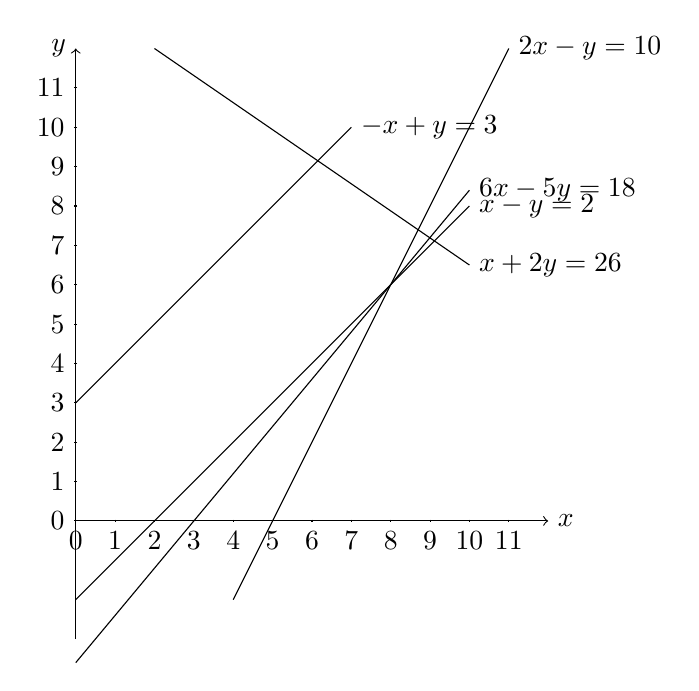
\begin{tikzpicture}[scale=0.5]
			\draw[->] (0,0) -- (12,0) node[below,right] {$x$};
			\draw[->] (0,-3) -- (0,12) node[above,left] {$y$};
			\draw (2,12) -- (10,6.5) node[above,right] {$x + 2y = 26$};
			\draw (0,3) -- (7,10) node[above,right] {$-x + y = 3$};
			\draw (0,-2) -- (10,8) node[above,right] {$x - y = 2$};
			\draw (4,-2) -- (11,12) node[above,right] {$2x - y = 10$};
			\draw (0,-3.6) -- (10,8.4) node[above,right] {$6x-5y = 18$};
			
			\foreach \x in {0,1,2,3,4,5,6,7,8,9,10,11}
			\draw (\x,1pt) -- (\x,-1pt) node[anchor=north] {$\x$};
			\foreach \y in {0,1,2,3,4,5,6,7,8,9,10,11}
			\draw (1pt,\y) -- (-1pt,\y) node[anchor=east] {$\y$};
			
		\end{tikzpicture}
	\end{center}
	
\end{frame}

\end{document}